\section{3D Reconstruction}\label{sec:reconstruction}

Having recovered the per-camera 2D trajectories, we lift them into a single 3D representation of the scene shared by all three cameras.

\subsection{Camera Calibration}
Intrinsic camera matrices are known a priori.
Extrinsic parameters are subsequently estimated by solving the Perspective-n-Point (PnP) problem, mapping manually annotated 2D image coordinates of court landmarks from the initial frame to their corresponding 3D world coordinates.
Lens distortion coefficients are integrated directly within the PnP optimization framework to ensure simultaneous rectification and alignment.

\subsection{Triangulation}
Detections are grouped by identity and frame index across the three cameras, then undistorted using the estimated intrinsics.
Players and the ball are reconstructed separately, since they move differently.

\subsubsection{Players}
Players are assumed to stand on the court floor.
Each camera's foot pixel is back-projected into a ray, and its intersection with the floor gives a ground position.
This constraint lets us localise a player even from a single view, which helps during occlusions.
Estimates from several cameras are merged by discarding outliers and averaging the rest.

%#TODO: Maybe i would avoid talking about DLT and SVD
\subsubsection{Ball}
The ball is airborne, so it cannot be tied to the floor.
Instead, its position is triangulated from the back-projected rays of all cameras that see it, requiring at least two views.
The rays are intersected with the Direct Linear Transform (DLT), which stacks the per-camera constraints into a homogeneous linear system and solves it via Singular Value Decomposition (SVD).
Views with a high reprojection error are discarded, and the point is re-triangulated from the rest.

\subsection{Trajectory Smoothing}
The triangulated trajectories still contain noise from detection jitter, calibration error, and outliers.
We smooth each one with a Kalman filter run forward in time, followed by a Rauch--Tung--Striebel (RTS) backward pass, so every point is corrected using both past and future observations.
Points that jump implausibly are rejected as outliers, and a trajectory is split whenever a gap grows too long, to avoid extrapolating across long occlusions.

\begin{figure}[h]
  \centering
  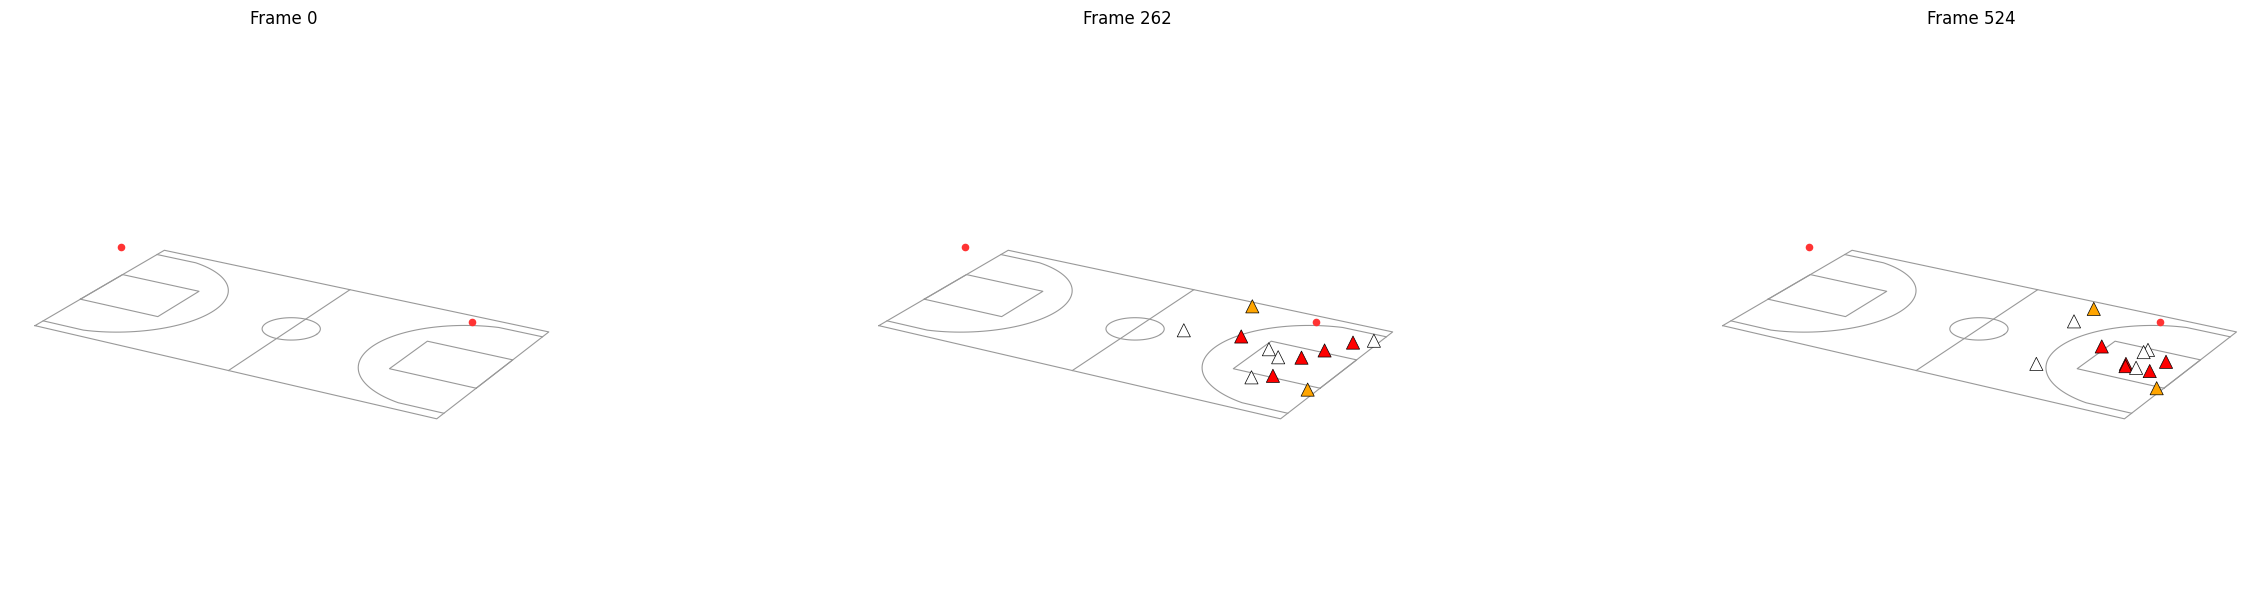
\includegraphics[width=\linewidth]{../media/fig_3d.png}
  \caption{Reconstructed 3D player and ball positions projected onto the court plane after RTS smoothing.}
  \label{fig:reconstruction}
\end{figure}
